\documentclass{beamer}
\usepackage[T1]{fontenc}
\usepackage{textcomp}
\usepackage[utf8x]{inputenc}
\usepackage[british]{babel}
\usepackage{url}
\usepackage{listings}
\usepackage{graphicx}
\usepackage{soul}

%FONT
\usepackage{palatino}              % font : palatino
\linespread{1.05}                  % Palatino needs more leading (space between lines)
\usepackage[sc]{mathpazo}

\title{Fitting an All-atom Protein Model to a $C_{\alpha}$-trace}
\subtitle{}

\author{Martin Dybdal \and Anders Boesen Lindbo Larsen \and Esben Skaarup}

\institute{\textrm{Datalogisk Institut, Københavns Universitet}}
\date{\today}

\mode<presentation>
{
  \usetheme{Frankfurt}
  %\usetheme{Warsaw} 
  \definecolor{uofsgreen}{rgb}{.125,.5,.25}
  \definecolor{natvidgreen}{rgb}{.196,.364,.239}
  \definecolor{kugrey}{rgb}{.4,.4,.4}
  \usecolortheme[named=uofsgreen]{structure}
  \usefonttheme[onlylarge]{structuresmallcapsserif}
  \usefonttheme[onlysmall]{structurebold}
}

\logo{
\includegraphics[height=1.5cm]{diku.png}}

\usenavigationsymbolstemplate{} % fjern navigation

\setcounter{tocdepth}{1}

\begin{document}

\frame{\titlepage}

% Martin
\section{Intro}
\subsection{bla}
\begin{frame}[t, fragile]
  \frametitle{bla} 
  \framesubtitle{subtitle}

  \begin{block}{blok}
    a
  \end{block}

  \pause

  \begin{itemize}
    \item 1
    \item 2
  \end{itemize}

\end{frame}

% Anders
\section{Backbone fitting}
\begin{frame}[t, fragile]
  \frametitle{Backbone fitting} 
%  \framesubtitle{subtitle}
\begin{center}
	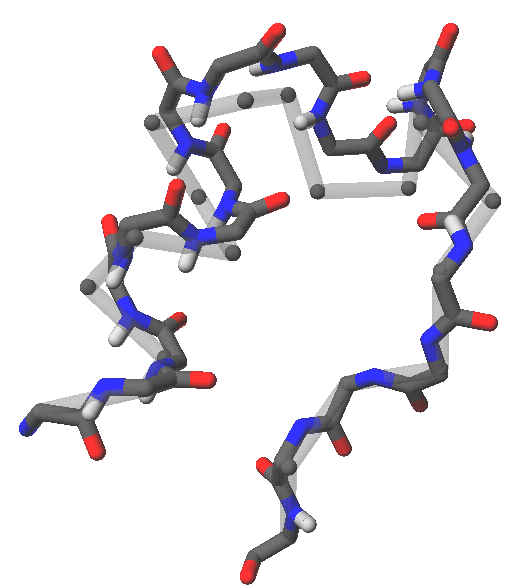
\includegraphics[width=.4\textwidth]{forside}
\end{center}
\end{frame}

\begin{frame}[t, fragile]
\frametitle{Backbone fitting} 
\framesubtitle{Cyclic coordinat descent}
\begin{center}
	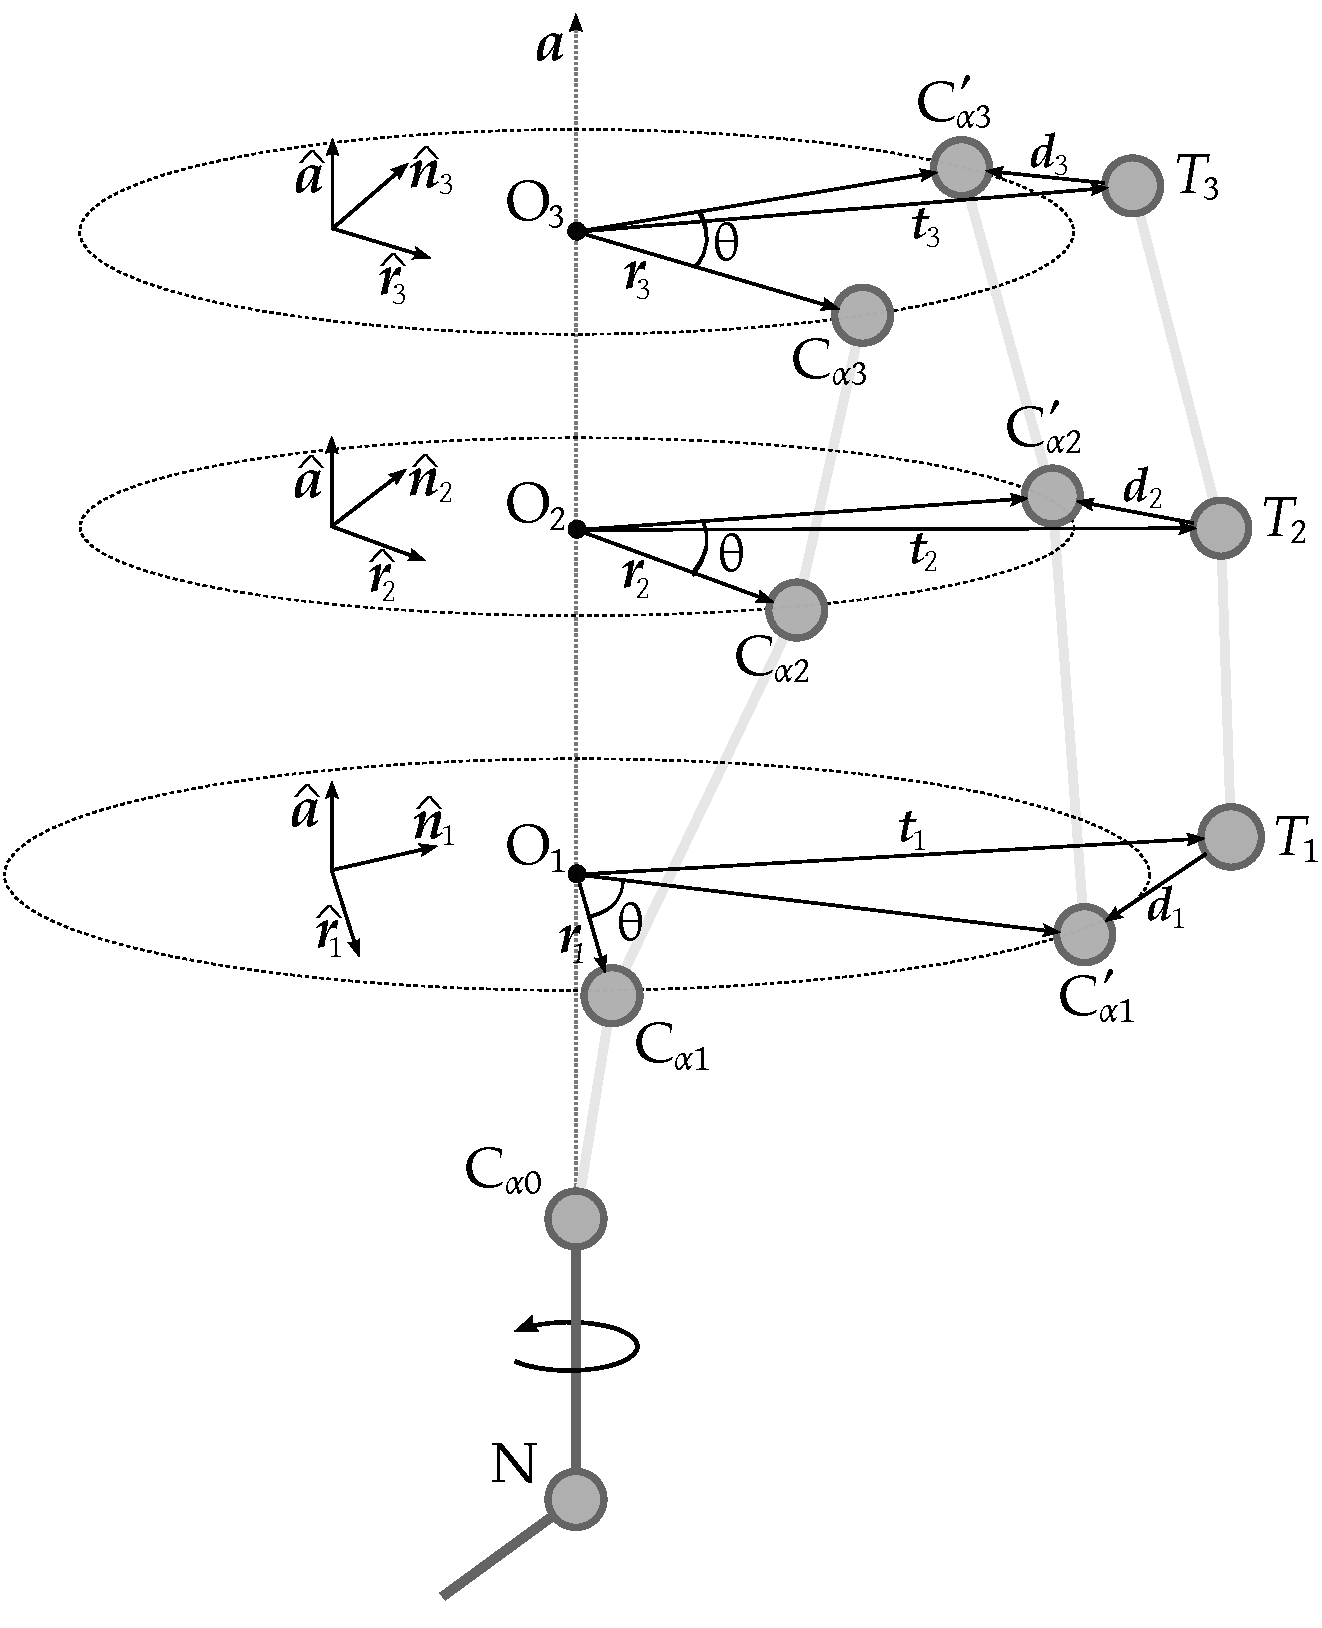
\includegraphics[width=.45\textwidth]{ccd}
\end{center}
\end{frame}

\begin{frame}[t, fragile]
\frametitle{Backbone fitting} 
\framesubtitle{Results}
\begin{columns}[c]
\column{2in}
\centering
Original\\
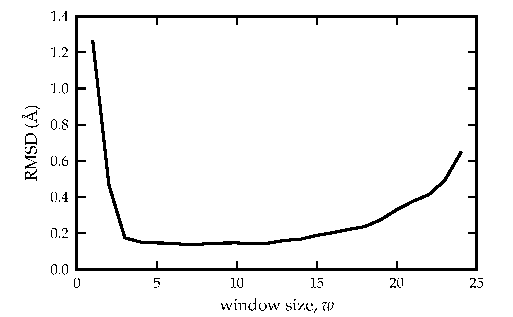
\includegraphics[width=1\columnwidth]{plot_rmsd}

\column{2in}
\centering
Fitted backbone\\
\hspace*{-.4cm}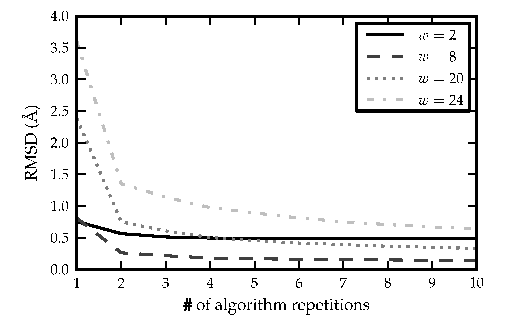
\includegraphics[width=1\columnwidth]{plot_rmsd_convergence}
\end{columns}
\end{frame}


\begin{frame}[t, fragile]
\frametitle{Backbone fitting} 
\framesubtitle{Results}
\begin{columns}[c]
\column{1.7in}
\centering
Original\\
\hspace*{-.33cm}
\includegraphics[width=1\columnwidth]{plot_ramachandran_orig}

\column{1.7in}
\centering
Fitted backbone\\
\hspace*{-.4cm}
\includegraphics[width=1\columnwidth]{plot_ramachandran}
\end{columns}
\end{frame}


% Esben


\end{document}
